% !TeX spellcheck = en_GB

\begin{comment}
\begin{itemize}
	\item goal == identify threats/attacks in KNX networks
	\item only a part in defence system
	\item attempt is to fit anomaly detection model best to normal behaviour in the network
	\item therefore it also necessary to account for usage cycles/periods/seasons of building usage
	\subitem since it has a direct impact on the bus activity
	\item changes in usage may be identified as anomaly -> which could also be interesting
	\subitem reflect e.g. physical intrusion, not intended use of the building, etc.
	\item ...
	
	\item novelty == in-band monitoring
		\subitem mention problems
	\item basic architecture according to \textcite{Pan2014}
	\item \enquote{Intrusion detection systems (IDSs) “are based on the beliefs that an intruder’s behavior will be noticeably different from that of a legitimate user and that many unauthorized actions are detectable” [2].} \parencite{Mukherjee1994,Yang2006}
	\item focus on inside attacks \enquote{The intruder has been granted access to the network and may have some knowledge about the network architecture, including where their targeted files or system vulnerabilities.} \parencite{Yang2006}
	
	\item only high level anomaly detection is done by algorithms, since simple measurements can be evaluated in Grafana
		\subitem e.g. change in packets per seconds
\end{itemize}
\end{comment}

\todo{better intro sentence?}
The overall goal is to identify and react to threats and attacks within \gls{bas} networks, which are indicated by malicious traffic.
This thesis attempts to solve on part of the problem by providing a framework to detect anomalies in those networks.
However, it is not part of this concept to identify the kind of attack, nor to distinguish it from abnormal network activity, caused by a rapid change of user behaviour.
Also it is to note, that the introduced system is merely a part in the defence line.

The architecture proposed in this section is inspired by \textcite{Pan2014}, with extensions made in regards for scalability and continuous use. (cf. Section~\ref{sec:concept:pipeline})
Opposed to \textcite{Pan2014}, which are using an inductive rule learning algorithm (cf. Chapter~\ref{sec:background:prior-work}), this work employs anomaly detection algorithm, which are able to be trained with unlabelled data sets. (cf. Section~\ref{sec:background:network:novelty})
This decision was made because \gls{bas} are mostly heterogeneous, since every building and its usage is different, compared to the fire detection system used by \textcite{Pan2014}.
Therefore, either the baseline model has to reflect a very broad \emph{normality}, or attacks are modelled as signatures. Later option has the drawback of requiring constant updates. Also a sufficiently large database of common attacks is required in first place.
Neither of these options seemed feasible.
Consequently, relying on anomaly detection algorithms made more sense in the provided context.
Despite anomaly based \glspl{ids} being highly useful in changing environments with possibly unknown threats (cf. Section~\ref{sec:background:network:ids:anomaly}), it is to note that they \enquote{are based on the beliefs that an intruder's behavior will be noticeably different from that of a legitimate user and that many unauthorized actions are detectable}. \parencite{Mukherjee1994,Yang2006}

\todo{better transition}
Further, to enable scalability and on-line detection, the proposed framework was designed around the message-passing design principle.
This allows for an easily scalable deployment, strongly capsules application modules, and handles recovery after crashes without data-loss.
Especially later two are not only desired characteristics of an production system, but also speed up development and testing rapidly.

Another novelty, compared to prior examples in literature (cf. Chapter~\ref{sec:background:prior-work}), is the focus of passing the flow-data from the Agent to the collector in-band. By doing so, there is no requirement for additional network wiring, which results in easier and possibly cheaper deployment for Agents across the network.
However, this also introduces new challenges, as the aggregated flow data needs to fit within a relatively small data package, in case of \gls{knx} 255 Bytes. (cf. Section~\ref{sec:background:bas:knx:proto:data})
Also, the collector and the analytical modules need to account for the fact, that no traffic from the Agents can pass the network, e.g. due to \gls{dos} attacks.

\todo{challenge, since there are no real flows.}
Another challenge arises from the nature of \gls{bas} itself. Unlike \gls{scada} networks, where actions follow strict rules and orders and are therefore highly predictable or \gls{ip} networks, which mostly transport connection based traffic. The communication in \gls{bas} networks consists of many short self-contained commands, which occur in seemingly random fashion, since they are mainly triggered by human behaviour. This includes (light) switches, \gls{pir} motion detectors, or door sensors.
Due to the fact, that most telegrams are short commands or status reports from sensors, there are no elaborative connection based communication flows in \gls{bas} networks, thus rendering flow-monitoring less useful.
To counteract this \hint{somewhat special} characteristic, the idea of flow-monitoring is interpreter rather liberal. 
Namely, by focussing more statistics of all telegrams or packets during a specific synchronised time window, instead of tracking individual flows, which also requires less resources on the Agent.

As already mentioned, this system can merely be a part of comprehensive security system. Acknowledging this fact, the outlier detection algorithms focus mainly on high level anomaly detection, as simpler measurements, like a change in telegrams per seconds, can be simply evaluated in a monitoring and alerting frontend like \gls{grafana}.

\section{Monitoring Pipeline}
\label{sec:concept:pipeline}

\begin{itemize}
	\item goal == monitor KNX traffic
	\item notion of \emph{project} is used to differentiate unique, not comparable KNX networks. Can be seen as a common prefix for everything which need to be named internally.
	\item monitoring should include the whole network/world view
	\item monitoring needs to be distributed, so Line Couplers can be configured properly
	\item monitoring is done by Agents
	\item Agents will send data gather over a time window to the collector (ref to neflow terminology)
	\item time windows of Agents are synchronised (by the collector) to make data analysis more reliable
	\item Agents send gathered data to collector via KNX network
	\item collector stores windows immediately in InfluxDB
	\item collector checks regularly the InfluxDB, if all Agents send in their time window
	\item if so the collector relays all windows, describing the same time slot (+/- a couple seconds), to the analyser modules
	\item if not all windows are in by specified timeout (10s or so) they are relayed anyway
	\item bundled windows are distributed by pub-sub-server independently to different analytical modules
	\item analytical modules compare the windows to a base-line model (in different fashions)
\end{itemize}

For the overall goal to identify threats and attacks within \gls{bas} networks by detecting anomalies, a reliable way to monitor packets or telegrams within said networks is required. Further, this data needs to be processed and analysed, for which a data-pipeline seems well suited.
In this section the general structure and flow within this pipeline is presented. (cf. Figure~\ref{fig:concept:architecture})

Within the here proposed pipeline the notion of a \emph{project} is used to differentiate unique, not comparable \gls{bas} networks, which share the same analytical resources. It can be understood as common prefix for all internal references. (cf. Chapter~\ref{sec:impl})
This is not only a beneficial option, when monitoring multiple networks one the same analytical infrastructure, but also allows for quick testing with different data-sets during development.
%To further improve use in production, as well as ease of development, ... (RabbitMQ, but this a detail for impl sec)

Following concepts in literature \parencite[cf.][]{Celeda2012,Pan2014} the pipeline is not build around analysing a full-take of traffic within a \gls{bas}, but rather follows the flow monitoring idea. (cf. Section~\ref{sec:background:network:netflow})
However, as stated above (cf. Chapter~\ref{sec:methods},~\ref{sec:concept}), traditional flow monitoring is well suited for \glspl{bas} like \gls{knx}. Therefore, the focus is on general statistical data of all packets or telegrams passing by an Agent within a specific time window.

Since one of the requirements for sufficiently efficient flow-monitoring is to obtain world view (cf. Section~\ref{sec:background:network:netflow},~\ref{sec:methods}), multiple flow monitoring Agents need to be distributed across the \gls{bas} network. Otherwise, network segmentation would be required to be switched off, so a central tapping point could be used for data acquisition.
Whereas this would decrease complexity, it is not advisable since segmentation is one of the fundamental security concepts e.g. in \gls{knx}. (cf. Section~\ref{sec:background:bas:knx:security})
Consequently, a number of Agents, distributed over the whole network, will gather statistical data and send it of to central service -- the Collector.

The Collector is not only responsible for receiving data from Agents and storing them in a database, but also synchronises these windows. Synchronising the windows simplifies the implementation of the analytical modules (cf. Section~\ref{sec:concept:anal}), since they do not need to account for distorted weights, introduced by changing overlaps or lengths of windows sent by the Agents.
This is archived, first of all by waiting until all windows from all Agents have been send to the Collector. Only then they are relayed to the analytical modules as one unit.
However, this only works reliable if the Agents are in sync with each other. If not the Collector would need to compensate for different, changing overlaps. Therefore another task of the Collector service is to ensure the Agents are synchronised, meaning the Agents capture the same length of the of statistical data in the same rhythm without shifting. \alert{rhythm is quite the right thing here, it's more a shift of the length...}
This is archived by communicating back to the Agent modules, regularly updating the \gls{rtc} and important settings like window length and a time point for starting new windows. (shift in time)

Regular two-way communication between Agents and Collector also has the benefit of identifying simple replay attacks (cf. Section~\ref{sec:methods}), since not or wrongly reacting to configuration requests can be detected.
Further, accounting for dynamic configuration of the agents allows for adjusting parameters based on the general network load.
E.g. the Collector could prolong the window length, when the \gls{bas} network is under heavy load to reduce additional traffic. Or the Collector could do the exact opposite to receive more detailed information on heavy resource utilisation.




\todo{figure, that shows how Agents are distributed in the network?}
\begin{figure}[h]
	\centering
	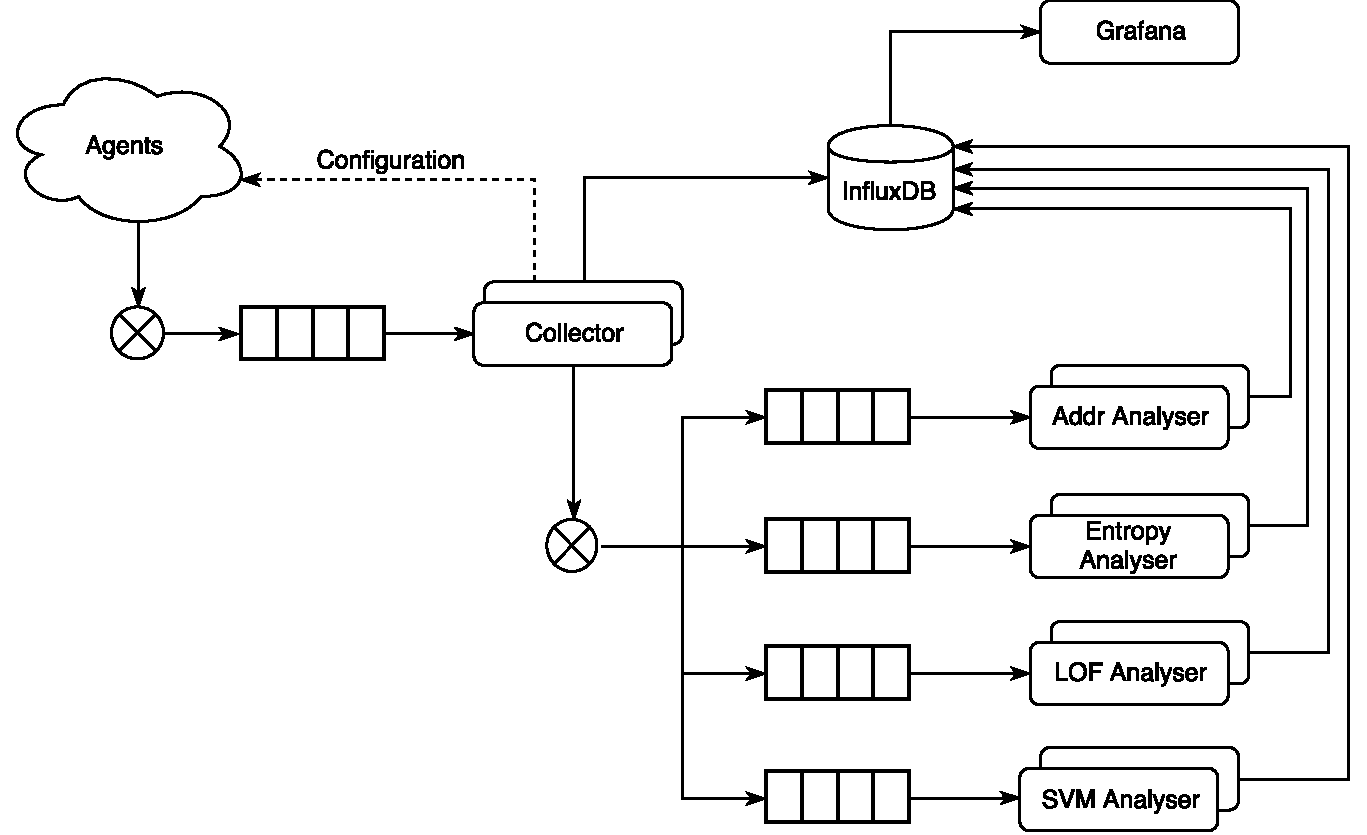
\includegraphics[width=\textwidth]{figures/300-concept-architecture.pdf}
	\caption[Pipeline Architecture]{Architecture of the monitoring pipeline \todo{explain symbols.} \todo{information flow back to agents, for time sync.}}
	\label{fig:concept:architecture}
\end{figure}

\section{Design of Netflow Agent}
\label{sec:concept:agent}

\begin{itemize}
	\item dedicated device
	\item sits in each or strategic important lines
	\item listens to bypassing traffic and aggregates it
	\item \alert{Critical to describe the difference to original netflow concept/idea here and why this decision was made}
		\subitem netflow is very IP oriented, where protocols include normally connections (TCP) or at least multiple steps/packets
		\subitem this provides a basis on which aggregation/grouping can be performed
		\subitem basically no flow (multi step protocols) in \gls{knx} during normal operation (besides configuration phase in \gls{knx})
		\subitem therefore gather statistical distribution of features on \gls{knx} \gls{telegram} over a given time span (window length)
		\subitem time span/window length should be configurable by the collector, so it can be adjusted according to network utilisation
		\subitem window length still needs to be synchronised among all agents to be able to use all aggregated agent windows in a world model
		\subitem further \gls{knx} can only transport 255 Bytes max in one telegram -> serious size restrictions
	\item after timeout gathered/aggregated data is send via \gls{knx} \gls{telegram} to the collector
	\item window consists
		\subitem meta data (timestamps, window lengths)
		\subitem absolute counter of how often an specific feature appeared in a window
			\begin{itemize}
				\item specific source address
				\item specific destination address
				\item apci value
				\item a specific payload length
				\item a specific \gls{hops}
			\end{itemize}
		\subitem checksum, and possibly signature
	\item window is encoded in a binary format to fit in the 255 Bytes
\end{itemize}

\section{The Collector Module}
\label{sec:concept:collector}

\begin{itemize}
	\item responsible for
		\subitem collecting data from agents through the \gls{knx} network
		\subitem storing raw time windows in \gls{influxdb}
		\subitem relaying raw, synchronised time windows to analytical modules
	\item listens to a single message queue containing time windows from all agents assigned to the same project
	\item agents must have unique names within one project
	\item windows are parsed and then submitted into the \gls{influxdb}, tagged with the agent-name and the project
	\item window is split into different measurements (tables) determined by the \gls{knx} fields observed.
	\item one additional measurement (table) \code{agent-status}, representing general status information
		\subitem timely length of the window
		\subitem end timestamp of the window
		\subitem boolean if window was relayed or not
	\item collector regularly checks the \gls{influxdb} for unrelayed windows (latest ones first)
	\item windows are grouped by time slot
	\item if all agents have submitted a window for a specific timeslot these windows are bundled and relayed to the analyser message exchange (cf.~Figure~\ref{fig:concept:architecture})
	\item for all successfully relayed windows set the \code{realayed} flag in the \code{agent-status} measurement to \code{true}
\end{itemize}

\section{Analyser Modules}
\label{sec:concept:anal}

\begin{itemize}
	\item 2 phases
	\item distinguished learning phase
	\item during learning phase the analyser module accesses directly the \gls{influxdb} for a specified time range
	\item group windows by time equal to the functionality of the collector
	\item construct \gls{vect} to train base model
	\item save base model in the filesystem
	
	\item during normal (analytical) operation
	\item accept grouped windows from collector via message exchange
	\item compares current window groups to base model to detect anomalies
	\item results of this analysis are stored back into the \gls{influxdb} as a separate \gls{idbmeasurement}
	
	\item multiple anomaly detection algorithms were considered
	\item according to \textcite{Lazarevic2003} \gls{lof}, NN, and unsupervised SVM perform the best
	\item \textcite{Eskin2002} suggests clustering and SVM as best performing algorithms
	\item ...
\end{itemize}

\subsection{The Address Analyser}
\label{sec:concept:anal:addr}

\begin{itemize}
	\item purpose is to detect new (novel) device addresses
	\item cf. new device attack
	\item during the learning phase it logs all occurring source and destination addresses per agent
	\item in the analytical phase it compares all source and destination addresses in a window with addresses (base model) accumulated in the training phase
	\item output \glspl{idbmeasurement}: \code{unknown\_src\_addr}, \code{unknown\_src\_telegrams}, \code{unknown\_dest\_addr}, \code{unknown\_dest\_telegrams}, \code{unknown\_addr}, \code{unknown\_telegrams}
\end{itemize}

\subsection{The Local Outlier Factor Analyser}
\label{sec:concept:anal:lof}

\begin{itemize}
	\item cf.~Section~\ref{sec:background:network:novelty:lof}
	\item proximity based technique (cf.~Section~\ref{sec:background:network:novelty:prox})
	\item tries to determine if a window represents normal behaviour
	\item both for local and world view
	\item builds feature vector out of
		\subitem normalized seconds since the beginning of the year
		\subitem source addresses
		\subitem destination addresses
		\subitem priority distribution
		\subitem hop count distribution
		\subitem payload length distribution
		\subitem \gls{apci} usage distribution
	\item time sensitivity/seasonal sensitivity is archived by including the relative timepoint in the current year
	\item training different model for different seasons is not necessary since \gls{lof} is a proximity base approach
\end{itemize}

\subsection{The Entropy Analyser}
\label{sec:concept:anal:entropy}

\begin{figure}[h]
	\centering
	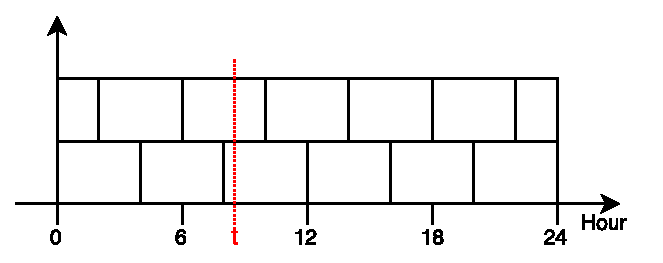
\includegraphics[]{figures/300-time-slots.pdf}
	\caption{Example of shifted time slots used in the entropy analyser module.}
	\label{fig:concept:time-slots}
\end{figure}

\begin{itemize}
	\item cf.~Section~\ref{sec:background:network:novelty:stat}
	\item statistical approach
	\item base model is trained using distribution of the \gls{pmf}
		\subitem determine statistical distribution per dimension in feature vector
	\item determine distribution for local (per agent) and world view
	\item to incorporate different seasons multiple base models are trained 
	\item the seasonal time range (day, week, year) is separated into slots
	\item amount of slots is doubled with half a slot length offset, so 2 slots apply per time point cf. Figure~\ref{fig:concept:time-slots}
	\item mitigates issues with artificial break on slot change
	\item feature vector
		\subitem source addresses
		\subitem destination addresses
		\subitem priority distribution
		\subitem hop count distribution
		\subitem payload length distribution
		\subitem \gls{apci} usage distribution
	\item entropy/information gain is calculated for the current distribution of the feature vector compared to the respectively base model
	\item individual entropies are summed up and stored in the \gls{influxdb} (additional to the individual entropies)
\end{itemize}

\section{Monitoring and Alerting}
\label{sec:concept:mon}

\begin{itemize}
	\item using \gls{grafana}
	\item visualise basic time series like amount of packets per agent
	\item visualise and monitor output from analyser modules
		\subitem should stay below certain threshold
	\item use internal alerting function
	\item benefits
		\subitem use existing, proven solution
		\subitem gain features for free (auth, alerting, graphing, etc)
		\subitem integrate with metrics from other sources
	\item decoupled from analyse modules
	\item good integration with \gls{influxdb}
\end{itemize}
